\chapter{Results} \label{chap:results}

To get an understanding of how the \Abb recommendation system performs relative to other techniques, the results will be presented in two sections. Section \ref{chap:results:sets} will compare the rule set learning system proposed in Chapter \ref{chap:algo} to Logistic Regression and Decision Trees. Section \ref{chap:results:rapid} will evaluate the \Abb system using the Lazy/Greedy approaches as well as using a \Abb system based on Linear Regression.


\section{Rule Set Performance}\label{chap:results:sets}

The rule set learning procedure from the \Abb system will be compared against Logistic Regression  \cite{hastie2009elements} and Decision Trees \cite{chen2016xgboost}. These techniques were briefly introduced in Chapter \ref{chap:intro} and \ref{chap:rl}. As mentioned in Section \ref{chap:algo:overview}, the \Abb system could make use of any machine learning system. This makes it important to directly compare the proposed inner rule set learner to other techniques.
Logistic Regression was chosen due to its prevalence in social and medical fields \cite{allegheny2019homeless} \cite{hong2018applications} \cite{toros2019early} and inherent interpretability.
Decision trees were chosen because of their similarity to classification rules. Decision Trees can be represented as rules, making them equally interpretable. The XGBoost library \cite{chen2016xgboost} was chosen to implement the Decision Trees. The XGBoost also supports Random Forests, which are an extension of Decision Trees (detailed in Chapter \ref{chap:rl}) that typically increase classifier performance. Using Random Forests from the XGBoost library is just as easy as using Decision Trees, so the below results will include a comparison to both Decision Trees and Random Forests.

Results will be presented with the confusion values first (True Positives, False Positives, True Negatives, and False Negatives). It is the author's preference to show these values as they present the full picture of classifier quality (and any quality metric can be derived from these four values, see Appendix \ref{chap:perf}). Precision, Sensitivity, and Specificity will also be presented for convenience. In general, the Precision and Sensitivity metrics will also be discussed as they neatly combine the confusion values and allow for the text to be more expressive.


\subsection{Baseline Algorithm Parameters}
The \Abb system generates rule sets based on multiple different time scales (values of $d$). However, this section will only compare the rule set learning used in \Abb, meaning only a single time scale can be used. In this section all three systems will be trained on and evaluated on a time scale of 30 days, that is, only a client's first 30 days since sleeping at the DI will be used. 
The rule set learning system of \Abb will use all the parameters discussed in Chapter \ref{chap:algo}.

All presented results are the averaged values from using 10-fold stratified cross-validation. 
The Logistic Regression was performed using the scikit-learn \footnote{scikit-learn version 0.20.3 obtained via pip} library implementation of Logistic Regression. As noted above XGBoost \footnote{XGBoost version 1.02 obtained via pip} was used for the Decision Tree and Random Forests implementations. In general, the default or recommended values were used for these systems, but for completeness Tables \ref{tbl:results:lrparam} and \ref{tbl:results:xgbparam} include all parameters used.

\begin{table}[h]
	\centering

	\begin{tabular}{lr}
	\toprule
	{Name} &    Value \\
	\midrule
	Solver & 'lbfgs' \\
	Max iterations & 1000 \\
	\bottomrule
	\end{tabular}

	\caption{Parameters used for the Logistic Regression model.}
	\label{tbl:results:lrparam}
\end{table}

\begin{table}[h]
	\centering

	\begin{tabular}{lr}
	\toprule
	{Name} &    Value \\
	\midrule
	max\_depth & 2, 5 \\
	objective & 'binary:logistic' \\
	\midrule
	colsample\_bynode & 0.8 \\
	learning\_rate & 1 \\
	num\_parallel\_tree & 100 \\
	subsample & 0.8 \\
	\bottomrule
	\end{tabular}

	\caption{Parameters used for the XGBoost Decision Trees and Random Forests. Values below the midline are specific to Random Forests.}
	\label{tbl:results:xgbparam}
\end{table}


\subsection{Minimum Lift Threshold} \label{chap:results:mlt}
As discussed in Section \ref{chap:algo:whypriori}, the Minimum Lift Threshold is a parameter of the rule set learning used by the \Abb system that allows the system designer to enforce a minimum Lift value for a rule set. Also discussed was the trade-off this imposes between rule set Precision and coverage (Sensitivity).
Figure \ref{fig:conf-sweep} displays this trade-off between Precision and Sensitivity by sweeping the Minimum Lift Threshold from 0.5 to the maximum possible lift value of 21 with 50 steps.
As can be seen, the Precision can only increase so far before the system fails to find rules that surpass the Minimum Lift Threshold. The reason that Precision moves in almost direct proportion to the Minimum Lift Threshold is that the Minimum Lift Threshold restricts the quality of rules that are added to the rule set. Thus, increasing the Minimum Lift Threshold will increase the Precision of the rule set. The corollary is that there will be fewer rules in the rule set, which will reduce the Sensitivity, as discussed in Section \ref{chap:rule:back}.
This relationship can be valuable for \Abb users because it will allow them to increase the Minimum Lift Threshold when high-quality rules that only identify a few individuals are desired. Conversely, it will allow the user to lower the threshold when they are willing to accept a lower Precision and desire a higher Sensitivity.


\begin{figure}[ht]
    \centering
    \figuretitle{Minimum Lift Threshold Sweep}
    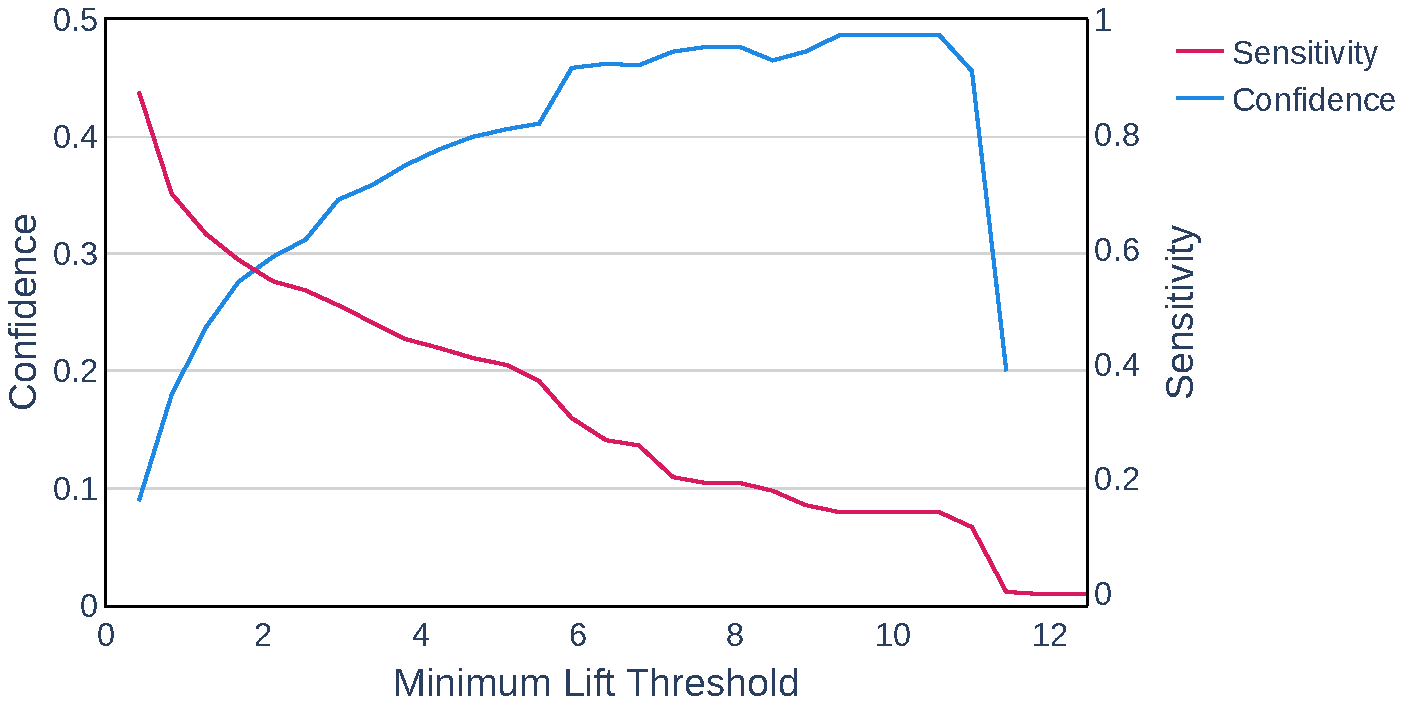
\includegraphics[width=1\textwidth]{Figures/Lift-Sweep.pdf}
		\caption{Demonstration of Precision and Sensitivity vs. Minimum Lift Threshold.}
    \label{fig:conf-sweep}
\end{figure}

\subsection{Results}


Table \ref{tbl:results:30} demonstrates the confusion values (with abbreviated column names) for the \Abb rule set learning system, Logistic Regression, Decision Trees, and the Random Forests model. 
There are three versions of the rule set learner presented here, each one with a different Minimum Lift Threshold (2.5, 6.4, 10.6). The values were chosen to roughly correspond to high, medium and low Precision based on Figure \ref{fig:conf-sweep}.
The exactness of the values used is a result of sweep analysis in Figure \ref{fig:conf-sweep}. That is, the sweep analysis used an even step on the Minimum Lift Threshold between values of 0.5 and 21, and the three Minimum Lift values were taken from those samples.
As can be seen in Table \ref{tbl:results:30}, increasing the Minimum Lift Threshold reduces the number of True Positives (and False Positives), but at the same time increases the Precision of the generated rule set. Thus, increasing the Minimum Lift Threshold presents a direct Precision/Sensitivity trade-off, as discussed in Section \ref{chap:results:mlt}.

Looking below at the other algorithms, it can be seen that the Logistic Regression performs similarly to the rule set learner with a Minimum Lift of 10.6 (outperforming slightly in both Precision and Sensitivity). The Random Forests (both depths) perform similarly to the rule set learner with a Minimum Lift of 2.5 (underperforming on Precision but outperforming on Sensitivity).
Logistic Regression outperforms the rule set learner with Minimum lift = 10.6 in both Precision and Sensitivity. This suggests that using Logistic Regression instead of an Apriori-based rule set learning could be beneficial especially when working in an environment where the Logistic Regression is understood. Section \ref{chap:results:rapid} includes a comparison of the \Abb system with an Apriori-based rule set learner, as well as one that uses Logistic Regression.

The Decision Trees and Random Forests classification results are presented in two variants, one with a maximum depth of 2, and one with a maximum depth of 5. This is done because the \Abb results are presented with a maximum depth of 2, but the Decision Tree/Random Forests models are capable of going to a larger depth within a reasonable amount of time. Table \ref{tbl:results:30} demonstrates that the increase in depth does not necessarily improve performance, as mentioned in Section \ref{chap:rl:tree}. As noted above, the Random Forests classifier does outperform the Decision Trees alone, however, neither classifier matches the Precision of the \Abb rule set learner or Logistic Regression.

As seen in Table \ref{tbl:results:30}, the performance of other classifiers can be roughly approximated with the \Abb rule set learner. Additionally, the performance trade-offs (Precision vs. Sensitivity) can be explicitly set. This is compared to using classifiers such as Logistic Regression that have an implicit trade-off. This is a tool that will be useful for users of the full \Abb system, as it can allow adjusting the Sensitivity in each time scale, thus allowing for more fine-grained control of which clients are identified. It is technically possible to adjust the Precision/Sensitivity of Logistic Regression and Tree based models, but that was not done here. The Logistic Regression and Tree based models all use the default training procedures according to their implementation. These default training procedures will have implicit Precision/Sensitivity trade offs which account for the differences seen here.

\begin{table}[h]
	\centering

	\begin{tabular}{p{0.3\textwidth}rrrrrrr}
	\toprule
	{Algorithm} &    TP &     FP &      TN &    FN &  Precision &  Sensitivity &  Specificity \\
	\midrule
	\Abb rule set learner (Minimum lift = 2.5) & 468 & 1032 & 16480 & 418 & 0.3120 & 0.5282 & 0.9411 \\
	\Abb rule set learner (Minimum lift = 6.4) & 237 & 276 & 17236 & 649 & 0.4620 & 0.2675 & 0.9842 \\
	% \Abb (0.224) & 364 & 547 & 16965 & 522 & 0.3996 & 0.4108 & 0.9688 \\
	\Abb rule set learner (Minimum lift = 10.6) & 126 & 133 & 17379 & 760 & 0.4865 & 0.1422 & 0.9924 \\
	Logistic Regression & 137 & 104 & 17408 & 749 & 0.5685 & 0.1546 & 0.9941 \\
	Decision Trees (Max depth = 2) & 541 & 1528 & 15984 & 345 & 0.2615 & 0.6106 & 0.9127 \\
	Decision Trees (Max depth = 5) & 536 & 1548 & 15964 & 350 & 0.2572 & 0.6050 & 0.9116 \\
	Random Forests (Max depth = 2) & 502 & 1139 & 16373 & 384 & 0.3059 & 0.5666 & 0.9350 \\
	Random Forests (Max depth = 5) & 504 & 1302 & 16210 & 382 & 0.2791 & 0.5688 & 0.9257 \\

	\bottomrule
	\end{tabular}

	\caption{Confusion values of the \Abb rule set learner, Logistic Regression, Decision Trees, and Random Forests.}
	\label{tbl:results:30}
\end{table}


\section{\Abb Performance} \label{chap:results:rapid}
As discussed in Chapter \ref{chap:algo} the Greedy and Lazy systems will be evaluated. The system that uses Logistic Regression in place of rule set learning will also be evaluated. This will be done by first showing the confusion values for each step as well as the summarized system performance. Then the MTTI values for each system will be compared against the DI definition from Chapter \ref{chap:data}.


\subsection{Greedy}
As discussed in Chapter \ref{chap:algo}, the Greedy system uses a different Minimum Lift Threshold for each time scale. Table \ref{tbl:results:mltgreedy} shows these Minimum Lift values. They were calculated by sweeping the Minimum Lift Threshold (see Figure \ref{fig:conf-sweep} for a visualisation) for each time scale and selecting the value that maximized the Precision of each rule set. As can be seen, as the value of $d$ increases the Minimum Lift Threshold increases as well. This is because as clients are in shelter longer, there is more data available to generate features, thus the rule set learner has a larger set of rules to pull from and can continue to generate rules even as the Minimum Lift Threshold gets large.

To get a rule set for each $d$, ten rule sets are generated using 10-fold stratified cross-validation. In most cases, the cross-validation procedure generates the same rule set 10 times, but in the case that more than one is generated, the single rule set generated the most times is selected for use. It is important to have a single generated rule set, because it will be used later in Section \ref{chap:results:rugresults}.

The rule sets used for the Greedy System are in Table \ref{tbl:results:greedysets}. Notably, none of the rule sets are made up of more than a single rule. This is because the Greedy system uses rule sets generated with the maximum possible Precision, that is, the Minimum Lift Threshold is increased until the rule set learning only returns the top rule. The introspection of a rule set, like the one in Table \ref{tbl:results:greedysets} is one of the primary benefits of using a rule learning system. That is, the rule set can be observed and analyzed after generation.
Table \ref{tbl:results:greedysets} demonstrates that at smaller time scales, Sleep and Age are the most important features. Larger time scales however show that Age becomes less important and exposure (or lack thereof) to DI counsellors becomes an important feature. These rule sets are thus useful to understand how classification decisions are made, but they also provide a tool that shelter staff can use to understand the features of a chronically homeless person.

\begin{table}[h]
	\centering

	\begin{tabular}{lr}
	\toprule
	{$d$} &  Minimum Lift \\
	\midrule
	7     & 6.4 \\
	14    & 7.2 \\
	30    & 9.3 \\
	61    & 9.3 \\
	91    & 10.2 \\

	\bottomrule
	\end{tabular}

	\caption{Minimum Lift Threshold values for the greedy system.}
	\label{tbl:results:mltgreedy}
\end{table}


\begin{table}[h]
	\centering

	\begin{tabular}{cc}
	\toprule
	$d$ & Rule Set \\
	\midrule
	7	& Age $\geq 59$ AND Sleep $\geq 7$ \\
	\midrule
	14	& Age $\geq 59$ AND Sleep $\geq 13$ \\
	\midrule
	30	& Age $\geq 59$ AND Sleep $\geq 27$ \\
	\midrule
	61	& EmployeeIsCounsellor $< 4$ AND Sleep $\geq 61$ \\
	\midrule
	91	& EmployeeIsCounsellor $< 6$ AND Sleep $\geq 91$ \\

	\bottomrule
	\end{tabular}

	\caption{The rule sets used in the Greedy System.}
	\label{tbl:results:greedysets}
\end{table}

% \begin{figure}[ht]
%     \centering
%     \figuretitle{Maximum Confidences}
%     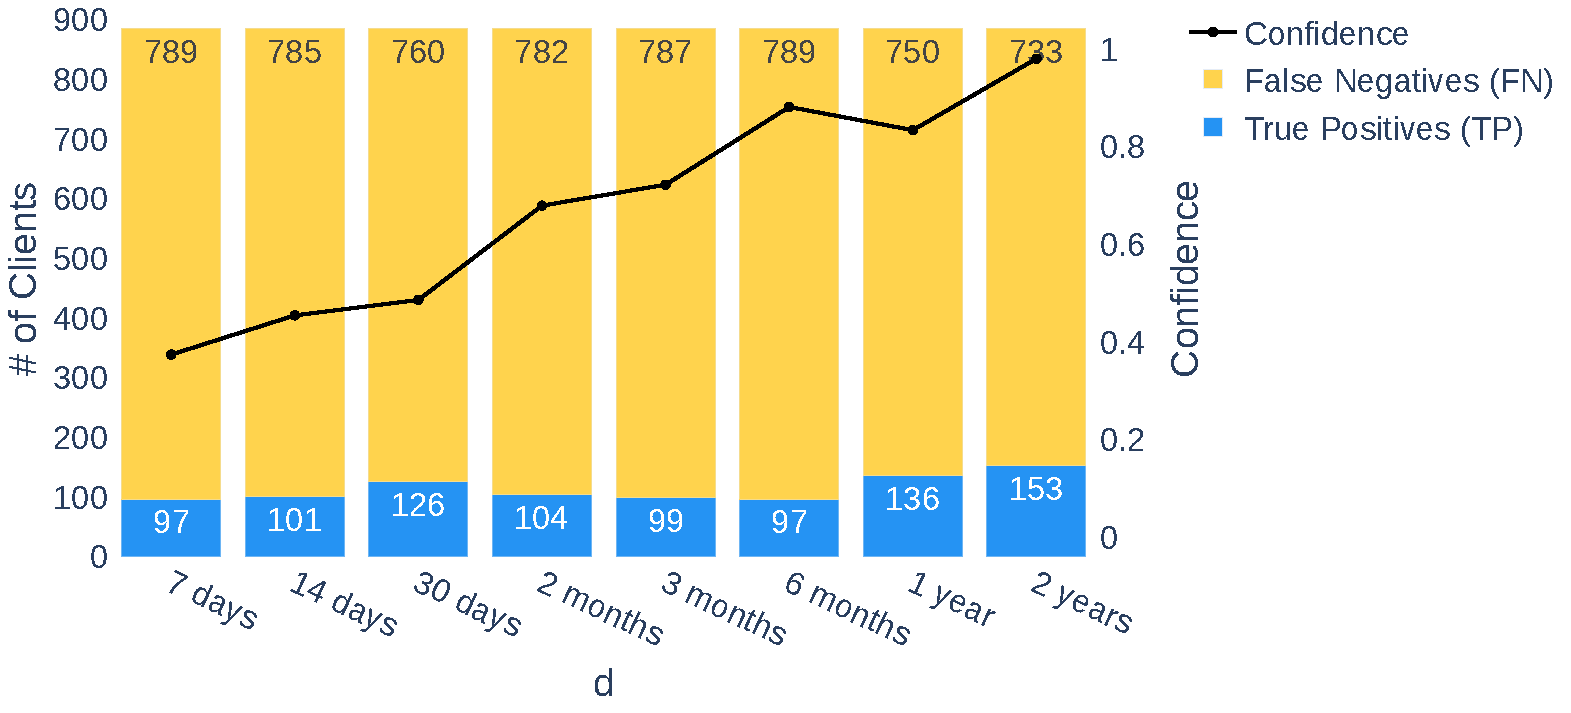
\includegraphics[width=1\textwidth]{Figures/Greedy-Columns.pdf}
% 		\caption{Confidence values taken from the rule set that maximizes Confidence at each time scale.}
%     \label{fig:greedycol}
% \end{figure}


\subsection{Lazy}

The Lazy system as introduced in Chapter \ref{chap:algo} uses a single Minimum Lift for all generated rule sets. For these results, a Minimum Lift of 6.4 is selected because it has a somewhat even trade-off between Precision and Sensitivity (Figure \ref{fig:conf-sweep} and Table \ref{tbl:results:30}). The rule set generation procedure is the same as used in the Greedy system.

Table \ref{tbl:results:lazysets} shows the rule sets used in the Lazy system. The most notable difference to the Greedy system is that the last three rule sets in the Lazy system have more than a single rule. The first two rule sets are the same in the Lazy and Greedy systems. This is because the first two Minimum Lift values used in the Greedy system are very close to the 6.4 used in the Lazy system (6.4 and 7.2, Table \ref{tbl:results:mltgreedy}). The last three rule sets all start with the same rule as the Greedy system, this is due to the behaviour of the Covering loop detailed in section \ref{chap:algo:weightcov}. Namely, that the rules are added to the rule set in order of highest Lift to lowest.

Some insights into the characteristics of chronic homelessness can be drawn from Table \ref{tbl:results:lazysets}. In particular, the importance of Sleep events on a chronic identification are very apparent. Another important observation is that individuals who have not met with a DI counsellor (or have few meetings) are more likely to become chronic. A different way of looking at this is that clients who have regular meetings with counsellors are more likely to become housed.

\begin{table}[h]
	\centering

	\begin{tabular}{cc}
	\toprule
	$d$ & Rule Set \\
	\midrule
	7 	& Age $\geq 59$ AND Sleep $\geq 7$ \\
	\midrule
	14	& Age $\geq 59$ AND Sleep $\geq 13$ \\
	\midrule
	30	& Age $\geq 59$ AND Sleep $\geq 27$ \\ 
			& No EmployeeIsCounsellor AND Sleep $\geq 29$ \\
			& Age $\geq 50$ AND Sleep $\geq 29$ \\
	\midrule
	61	& EmployeeIsCounsellor $< 4$ AND Sleep $\geq 61$ \\
			& Age $\geq 50$ AND Sleep $\geq 38$ \\
	\midrule
	91	& EmployeeIsCounsellor $< 6$ AND Sleep $\geq 91$ \\
			& Age $\geq 59$ AND Sleep $\geq 55$ \\
			& Age $\geq 50$ AND Sleep $\geq 55$ \\
	\bottomrule
	\end{tabular}

	\caption{The rule sets used in the Lazy System.}
	\label{tbl:results:lazysets}
\end{table}

% \begin{figure}[ht]
%     \centering
%     \figuretitle{Confidences at Minimum Lift of 6.4}
%     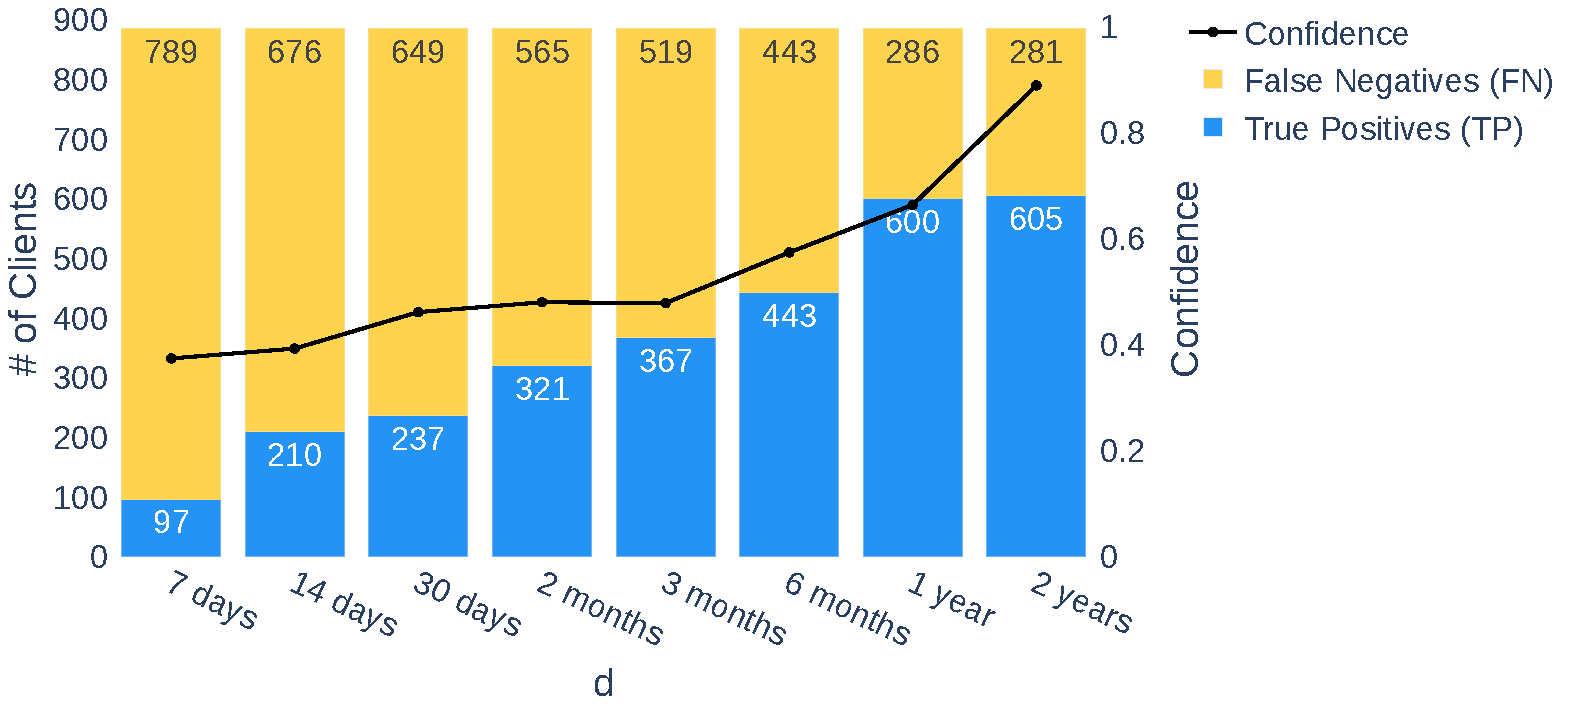
\includegraphics[width=1\textwidth]{Figures/Lazy-Columns.pdf}
% 		\caption{Confidence values taken from rule sets with Minimum Lift of 6.4.}
%     \label{fig:lazycol}
% \end{figure}

\subsection{Logistic Regression}
The Logistic Regression was integrated into the \Abb system by swapping out the Weighted Covering Algorithm rule set learner for Logistic Regression. This meant that five Logistic Regression models were trained (for five different values of $d$) and tested. 
Logistic Regression does not generate a model that can easily be saved and compared (like in rule set learning). The results presented in Section \ref{chap:results:rugresults} depend on having five trained models which were selected from a set of 10 trained by 10-fold stratified cross-validation. That is not possible with Linear Regression so instead, a simple 50-50 train/test split was performed. The model was trained on one split but evaluated on the entire dataset. This was done to ensure the numbers would line up with the other models.

% \begin{figure}[ht]
%     \centering
%     \figuretitle{Confidences using Logistic Regression}
%     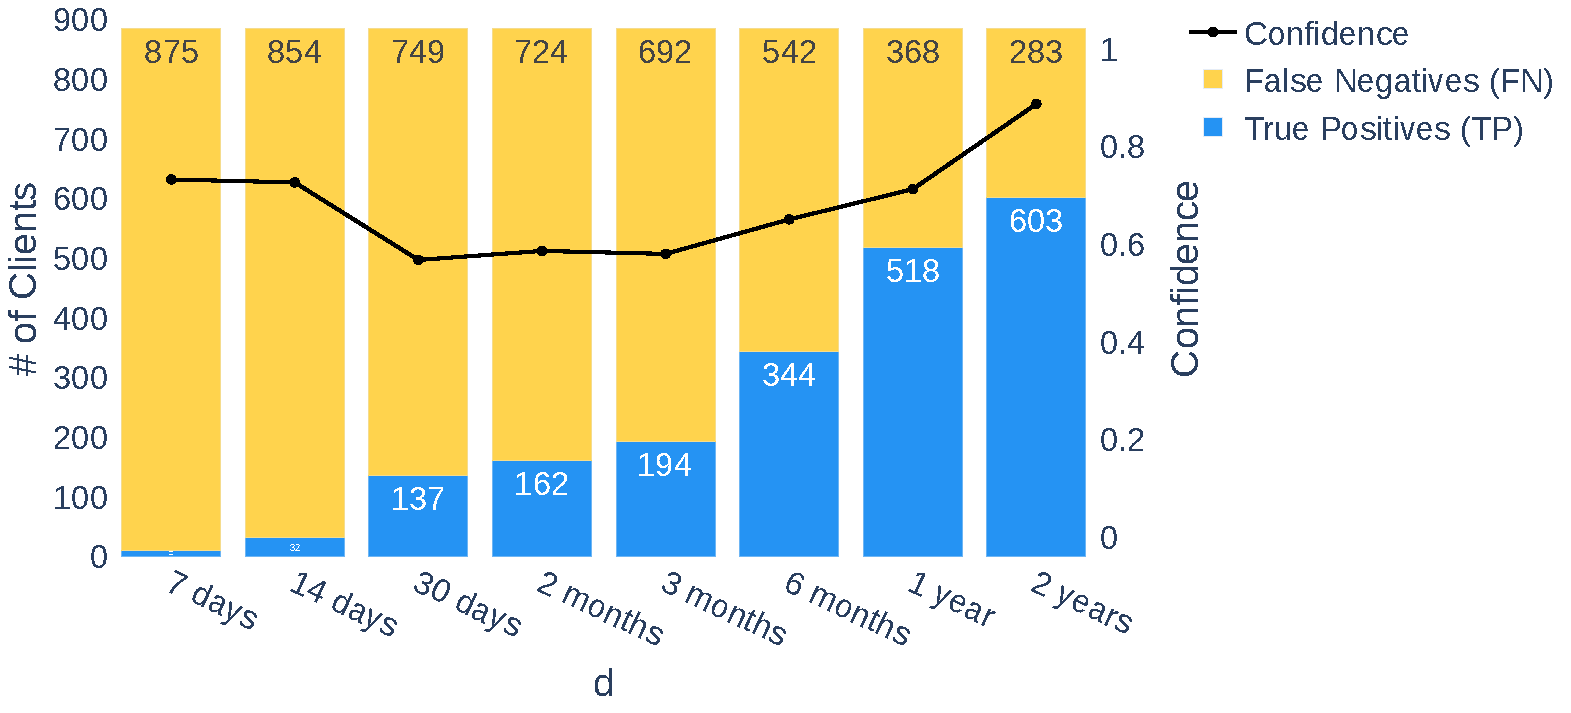
\includegraphics[width=1\textwidth]{Figures/LR-Columns.pdf}
% 		\caption{Confidence values taken from using Logistic Regression instead of rule set learning.}
%     \label{fig:lrcol}
% \end{figure}

\subsection{Results} \label{chap:results:rugresults}

Table \ref{tbl:results:abb} presents the results of the Greedy/Lazy systems and the Logistic Regression system.
In these results, the confusion values are presented without overlap between rule sets. What that means is that clients who are identified by one rule set (e.g. $d=7$) will be removed from the data set. This allows the Final row to be presented without over-inflating the number of individuals identified by the system. It also demonstrates the degree to which the generated rule sets do overlap. To display this removal, Table \ref{tbl:results:abb} has a new column, $N$, which is the cumulative sum of correctly identified individuals.

The Greedy system performs comparably to the single rule set with a Minimum Lift of 6.4 (Table \ref{tbl:results:30}). The benefit of the Greedy system can be seen by observing the distribution of the True Positive values with respect to the time scales. That is, the majority of clients (more than 100) are identified in fewer than 30 days (an average of around 29 days), with most of the rest being identified after 61 days. This is due to the overlap between the rule sets with short time scales, and rule sets with larger time scales. The rule sets with shorter time scales identify chronic clients early on, and those clients are then removed from the data set used by the rule sets with larger time scales, resulting in less identified clients. This is demonstrated in Table \ref{tbl:results:greedysets} where it can be seen that the rule sets generated at different time scales are similar. This is an example of the transparency that makes rule set based classifiers useful.

The Lazy system does not suffer the Sensitivity fall off quite as sharply as the Greedy system. This means that only about a third of identified clients are identified in less than 30 days (clients are identified after an average of around 33 days), and the rest are identified at a later time scale. There are about twice as many True Positives identified by the Lazy system, and this comes at the cost of having a little more than twice as many False Positives. The Lazy system also demonstrates the overlap, particularly at $d=14$ and $d=91$ where the Sensitivity is very low.

Comparing the results of the Lazy system with Table \ref{tbl:results:30}, it can be seen that the Lazy system performs somewhere between the single rule sets with Minimum Lift values of 2.5 and 6.4. The results of the Lazy system however have a more favourable Precision/Sensitivity trade-off, with Precision and Sensitivity being near the higher end of either single rule set scenario. Same as with the Greedy system, the real benefit of the Lazy system is that many of the clients are identified in two weeks or less.

The Logistic Regression system performs quite similar to the single time scale results presented in Table \ref{tbl:results:30}. The Precision is approximately the same but the Sensitivity has improved by approximately 50\%. This Sensitivity increase comes from the redundancy of having five rule sets. Notably, the Linear Regression based system does not appear experience the Sensitivity falloff quite as sharply as the other two systems. The clients are identified at more even intervals, with a mean around 46 days. This appears to happen for two reasons. The first being that the Linear Regression system has a much lower Sensitivity at $d=7$ days, meaning that the overlap will be less pronounced as it is spread out more. The second is that the Linear Regression system is possibly training models that have less overlap than the rule set based systems. 

Overall there is no superior system based on Table \ref{tbl:results:abb}. All systems present a new set of Precision/Sensitivity trade-offs and can situationally fit a user's needs depending on what those needs currently are. While it seems that both systems improved the rapid identification situation when compared to the single rule sets in Table \ref{tbl:results:30}, it is not exactly clear. In the following section, the MTTI metric will be used to compare the rapidity of identification.

\begin{table}[h]
	\centering

	\begin{tabular}{lrrrrrrrr}
	\toprule
	{$d$} &    $N$ &   TP &   FP &     TN &   FN &  Precision &  Sensitivity &  Specificity \\
	\midrule
	\toprule
	Greedy & & & & & & & & \\
	\midrule
	7     &   95 &   95 &  150 &  17362 &  791 &    0.387755 &     0.107223 &     0.991434 \\
	14    &  109 &   14 &   16 &  17346 &  777 &    0.466667 &     0.017699 &     0.999078 \\
	30    &  115 &    6 &   11 &  17335 &  771 &    0.352941 &     0.007722 &     0.999366 \\
	61    &  183 &   68 &   42 &  17293 &  703 &    0.618182 &     0.088197 &     0.997577 \\
	91    &  186 &    3 &    9 &  17284 &  700 &    0.250000 &     0.004267 &     0.999480 \\
	Final &  186 &  186 &  228 &  17284 &  700 &    0.449275 &     0.209932 &     0.986980 \\
	\bottomrule
	\toprule
	Lazy & & & & & & & & \\
	\midrule
	7     &   95 &   95 &  150 &  17362 &  791 &    0.387755 &     0.107223 &     0.991434 \\
	14    &  109 &   14 &   16 &  17346 &  777 &    0.466667 &     0.017699 &     0.999078 \\
	30    &  264 &  155 &  195 &  17151 &  622 &    0.442857 &     0.199485 &     0.988758 \\
	61    &  366 &  102 &  157 &  16994 &  520 &    0.393822 &     0.163987 &     0.990846 \\
	91    &  373 &    7 &   21 &  16973 &  513 &    0.250000 &     0.013462 &     0.998764 \\
	Final &  373 &  373 &  539 &  16973 &  513 &    0.408991 &     0.420993 &     0.969221 \\
	\bottomrule
	\toprule
	Logistic Regression & & & & & & & & \\
	\midrule
	7     &   20 &   20 &    9 &  17503 &  866 &    0.689655 &     0.022573 &     0.999486 \\
	14    &   35 &   15 &    3 &  17500 &  851 &    0.833333 &     0.017321 &     0.999829 \\
	30    &  115 &   80 &   56 &  17444 &  771 &    0.588235 &     0.094007 &     0.996800 \\
	61    &  173 &   58 &   50 &  17394 &  713 &    0.537037 &     0.075227 &     0.997134 \\
	91    &  208 &   35 &   36 &  17358 &  678 &    0.492958 &     0.049088 &     0.997930 \\
	Final &  208 &  208 &  154 &  17358 &  678 &    0.574586 &     0.234763 &     0.991206 \\
	\bottomrule
	\end{tabular}

	\caption{Performance of the \Abb systems.}
	\label{tbl:results:abb}
\end{table}


\subsection{Mean Time To Identification}

The MTTI is a tool introduced in Chapter \ref{chap:algo} for comparing the rapidity of identification. This tool has been used with the Greedy, Lazy, and Logistic Regression systems.


The MTTI provides the mean time for all chronic clients to be identified as such. This means that clients that are not identified as chronic by the \Abb systems will still need to be identified by the DI definition. This results in MTTI values with a large number of days. To demonstrate how these systems compare on the clients they are able to identify, two new metrics are presented. The first is AIT, or Average Identification Time, which is the average time to identification for chronic clients who are identified by a system. The other is the Median Identification Time, which takes the median time to identification, rather than average. Total number of identified clients $N$ will be presented as well.

Table \ref{tbl:results:mtti} presents the MTTI values for the Greedy/Lazy systems, the Logistic Regression system, a system that uses a single rule set trained on 30 days (with a Minimum Threshold of 6.4), and using just the DI definition to classify individuals.
As stated in Section \ref{chap:algo:mtti}, the MTTI is the Mean Time to Identification for the 886 chronic clients in the data set. When a client is not identified by any of the classifier systems, the remaining unclassified individuals are assumed to be identified by the DI chronic definition after 666 days. The result of this is that all MTTI values are perhaps unexpectedly large. When evaluating a system based on MTTI, it is important to observe how many days less the MTTI value is when compared against the DI definition. The AIT and MIT values cover only the correctly identified future chronic individuals, they give a reference to how rapidly each system successfully identifies clients.
The Greedy system performs the worst of the four classifiers tested with the Logistic Regression system performing very similarly. The Lazy system performs the best, and the single time scale classifier performs somewhere in between. Looking back at Tables \ref{tbl:results:abb} and \ref{tbl:results:30} it appears that the reason for this relates with the Sensitivity of each system, having values of 0.21, 0.42, 0.23, and 0.27 respectively.
Another aspect of the Logistic Regression system that increased the MTTI value is the distribution of Sensitivity as seen in Table \ref{tbl:results:abb}. Logistic Regression has a fairly even distribution of Sensitivity compared to the Greedy and Lazy systems which would can be seen to increase the AIT by 15 days. 
This result suggests that the best way to identify individuals rapidly is to widen the net and allow many individuals to be identified at the cost of Precision.
This result may also seem to suggest that the Greedy and Logistic Regression systems have poor performance, however, they require half the amount of housing resources as the Lazy system and still reduce the MTTI by over 100 days when compared to the DI definition alone. This could be a very useful heuristic for homeless shelters to use when housing resources are limited.


\begin{table}[h]
	\centering

	\begin{tabular}{lrrrr}
	\toprule
	{System} &  MTTI (days) & AIT (days) & MIT (days) & $N$ \\
	\midrule
	Greedy & 532 & 29.4 & 7 & 186 \\
	Lazy & 400 & 33.2 & 30 & 373 \\
	Logistic Regression & 520 & 45.5 & 30 & 208 \\
	$d=30$ & 496 & 30 & 30 & 237 \\
	DI Definition & 666 & 666 & 349 & 886 \\

	\bottomrule
	\end{tabular}

	\caption{The calculated MTTI values.}
	\label{tbl:results:mtti}
\end{table}

% \section{Demographics} \label{chap:results:demographics}
% \tdo{Discuss the need for looking at demographics}
% - definitions take a single slice of demographics, this can be more accurate
% \tdo{Display the demographic analysis results}

% \begin{table}[h]
% 	\centering

% 	\begin{tabular}{llll}
% 	\toprule
% 	{} &       min &      max &   median \\
% 	\midrule
% 	Age                          &        19 &       85 &       58 \\
% 	Bar (Count)                  &         0 &       55 &        0 \\
% 	CounsellorsNotes (Count)     &         0 &      443 &        7 \\
% 	EmployeeIsCounsellor (Count) &         0 &      464 &       11 \\
% 	EmsLogFlag (Count)           &         0 &       24 &        0 \\
% 	Log (Count)                  &         0 &     2419 &        8 \\
% 	PoliceLogFlag (Count)        &         0 &        8 &        0 \\
% 	ProgressDetails (Count)      &         0 &      539 &       13 \\
% 	Sleep (Count)                &         7 &     3380 &    243.5 \\
% 	Interactions (Count)         &         7 &     4517 &    354.5 \\
% 	Tenure (Days)                &         7 &     3733 &    696.5 \\
% 	Usage (\%)                    &  0.460678 &      100 &  78.2731 \\
% 	Average Gap Length (Days)    &  0.991935 &  233.692 &   1.2782 \\
% 	Stays (Count)                &         7 &     3380 &    243.5 \\
% 	Episodes (Count)             &         1 &       21 &        2 \\
% 	\bottomrule
% 	\end{tabular}

% 	\caption{}
% 	\label{tbl:results:demo}
% \end{table}



\section{Summary}

This chapter demonstrated the results of the \Abb system and compared those results against some more commonly used classification systems. These results demonstrated that the \Abb rule set learning system performs comparably to the standard interpretable classifiers. Additionally, the \Abb rule set learning is easily configurable to adjust the balance between Precision and Sensitivity.

The MTTI metric was used to compare the Greedy/Lazy \Abb systems with a Logistic Regression based \Abb system. This demonstrated that Sensitivity is the most important metric when it comes to rapid identifications, but low Sensitivity classifiers can still be beneficial.

Overall the \Abb systems perform comparably to other classification systems but with an easy-to-understand set of steps and a clear/interpretable resulting model (rule sets). 